  \documentclass[12pt]{article}
 
\usepackage[margin=1in]{geometry}
\usepackage{amsmath,amsthm,amssymb}
\usepackage[spanish]{babel}
\decimalpoint
\usepackage[utf8]{inputenc}
\usepackage{enumitem, kantlipsum}
\usepackage{graphicx}
\newcommand{\angstrom}{\mbox{\normalfont\AA}}
\setlength{\parindent}{0cm} 

\begin{document}
 
\begin{center}
\Large \textbf{C.Física Moderna: Taller 8}\\
\normalsize \textbf{Longitud de onda de De-Broglie, experimento de Davisson-Germer y de Frank-Hertz}
\end{center}
 
  

\section{Longitud de onda de De-Broglie }



\begin{enumerate}
	\item Calcule la longitud de onda de De-Broglie de un cuerpo de masa 100 kg moviéndose a $0.5c$.
	\item Calcule la longitud de onda de De-Broglie de un electrón que es acelerado por una diferencia de potencial de 5V.
	\item Compare las longitudes de onda obtenidas y concluya sobre la longitud de onda para objetos macroscópicos.
\end{enumerate}

\noindent\rule{16.5cm}{0.4pt}





\section{Experimento de Davisson-Germer}

 En el experimento de Davisson-Germer se aceleran electrones mediante un potencial $V$, y luego
se hace incidir estos electrones sobre un cristal. Dado que la longitud de onda asociada de Broglie de los
electrones es del orden de la longitud de separación de los planos del cristal, los electrones son
difractados.

\begin{enumerate}
	\item Encuentre  la relación entre las posiciones donde se detecta una mayor intensidad de electrones
	detectados y el voltaje de aceleración.
	\item Para un voltaje de aceleración de 54 V, establezca la primera posición donde se detectará una
	mayor intensidad de electrones para un cristal con distancia interplanar de 0.092 nm.
\end{enumerate}

\noindent\rule{16.5cm}{0.4pt}

\section{Experimento de Frank-Hertz}

En el experimento de Frank-Hertz se hace fluir corriente eléctrica sobre un tubo que contiene
vapor de mercurio, el nivel de corriente se controla con un voltaje variable de aceleración entre el
cátodo A y una rejilla, la corriente se mide entre la rejilla y el cátodo B, en el cual se mantiene un
pequeño voltaje de frenado constante. La gráfica de corriente versus voltaje en el tubo, se muestra
a continuación, donde se muestra una caída abrupta de la corriente para 4.9 V, 9.8 V, 14.7 V.

	\begin{figure}[h!]
		\centering
	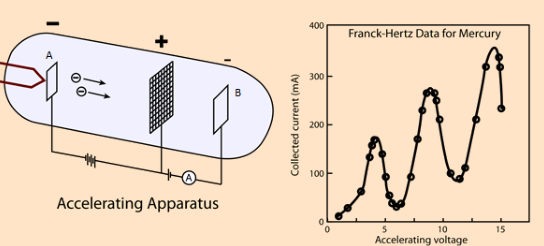
\includegraphics[scale=1, angle=0]{frank}
	\caption{Figuras tomadas de HyperPhysics}
\end{figure}

\begin{enumerate}
	\item Explicar en términos de colisiones elásticas e inelásticas entre los electrones y los átomos de
	mercurio el resultado de esta gráfica.
	\item  Determinar frecuencia y longitud de onda de la radiación electromagnética emitida por el átomo
	de mercurio para la transición entre el estado base y el primer nivel de energía.
	\item Suponga que se llena ahora el tubo con hidrógeno. ¿Para qué voltaje de aceleración espera que la
	corriente caiga de forma abrupta?
\end{enumerate}

\noindent\rule{16.5cm}{0.4pt}








\begin{center}
	\textbf{Fórmulas útiles}
\end{center}

Longitud de onda de De-Broglie:

\begin{equation*}
\lambda = \frac{h}{p}
\end{equation*}

Ley de Bragg:

\begin{equation}
n\lambda = 2 d \sin\theta
\end{equation}

Energías permitidas del átomo de hidrógeno:

\begin{equation*}
E_n = - \frac{13.6}{n^2} \text{eV}
\end{equation*}


\end{document}